\chapter{Machine Learning}

\section{Artificial Neural Networks}

\textit{Artificial Neural Networks} are mathematical models inspired by biological neural networks. They are composed of (layers of) connected neurons and characterized by processes changing their structure based on the flowing information during the \textit{learning} stage.

The first mention of this term is in McCulloch and Pitts' 1943 work \cite{McCulloch1943}, where they introduced a Threshold Logic Unit (or Linear Threshold Unit), able to implement simple boolean functions \ref{fig:TLU}.

\begin{figure}[H]
	\centering
	\begin{equation*}
		\begin{aligned}[c]
			TLU(\vec{x}) & = \phi \bigg( \sum_{i=1}^{n}{w_{i} \cdot x_{i}} \bigg) \\
			\phi(x)      & = x - \theta \geq 0
		\end{aligned}
		\quad
		\begin{aligned}[c]
			n      & = 2   \\
			\theta & = 1.5 \\
		\end{aligned}
		\quad
		\begin{aligned}[c]
			w_{1} & = 1.0 \\
			w_{2} & = 1.0
		\end{aligned}
	\end{equation*}
	\caption{Boolean logic AND implemented by a Threshold Logic Unit}
	\label{fig:TLU}
\end{figure}

\paragraph{Perceptron}

Rosenblatt introduced in 1958 the \textit{Perceptron}\cite{rosenblatt1958perceptron}, a linear binary classificator now considered the simplest feed-forward neural network.

It can be modeled as follows:

\begin{equation*}
	\begin{aligned}[c]
		f(\mathbf{x}) = \begin{cases}1 & \text{if }\ \mathbf{w} \cdot \mathbf{x} + b > 0,\\0 & \text{otherwise}\end{cases}
	\end{aligned}
\end{equation*}

\begin{equation*}
	\begin{aligned}[c]
		w = \begin{bmatrix}
			w_{1} & \cdots & w_{d} & b
		\end{bmatrix}
	\end{aligned}
	\quad
	\begin{aligned}[c]
		\vec{x} = \begin{bmatrix}
			x_{1}  \\
			\vdots \\
			x_{d}  \\
			1
		\end{bmatrix}
	\end{aligned}
\end{equation*}

\begin{figure}[H]
	\centering
	\begin{tikzpicture}
		\node[functions] (center) {};
		\node[below of=center,font=\scriptsize,text width=4em] {Activation function};
		\draw[thick] (0.5em,0.5em) -- (0,0.5em) -- (0,-0.5em) -- (-0.5em,-0.5em);
		\draw (0em,0.75em) -- (0em,-0.75em);
		\draw (0.75em,0em) -- (-0.75em,0em);
		\node[right of=center] (right) {};
		\path[draw,->] (center) -- (right);
		\node[functions,left=3em of center] (left) {$\sum$};
		\path[draw,->] (left) -- (center);
		\node[weights,left=3em of left] (2) {$w_2$} -- (2) node[input,left of=2] (l2) {$x_2$};
		\path[draw,->] (l2) -- (2);
		\path[draw,->] (2) -- (left);
		\node[below of=2] (dots) {$\vdots$} -- (dots) node[left of=dots] (ldots) {$\vdots$};
		\node[weights,below of=dots] (n) {$w_n$} -- (n) node[input,left of=n] (ln) {$x_n$};
		\path[draw,->] (ln) -- (n);
		\path[draw,->] (n) -- (left);
		\node[weights,above of=2] (1) {$w_1$} -- (1) node[input,left of=1] (l1) {$x_1$};
		\path[draw,->] (l1) -- (1);
		\path[draw,->] (1) -- (left);
		\node[weights,above of=1] (0) {$w_0$} -- (0) node[input,left of=0] (l0) {$1$};
		\path[draw,->] (l0) -- (0);
		\path[draw,->] (0) -- (left);
		\node[below of=ln,font=\scriptsize] {Inputs};
		\node[below of=n,font=\scriptsize] {Weights};
	\end{tikzpicture}
\end{figure}

\section{Activation Functions}

The choice of activation functions in neural networks affects the training dynamics and the final performance. A lot of alternatives have been proposed and are in development, but none managed to reach the popularity of ReLU.

\begin{description}[align=right,leftmargin=*,labelindent=5cm]
	\item[Sigmoid (Logistic)]
	      ${(1 + e^{-x})}^{-1}$
	\item[Hyperbolic]
	      $\tanh(x)$
	\item[Rectified Linear Unit (ReLU)]
	      $\max(0,\, x)$
	\item[Leaky ReLU]
	      $\max(0.01x,\, x)$
	\item[Parametric LReLU]
	      $\begin{cases}
			      \alpha x & \text{if } x \geq 0 \\
			      x        & \text{if } x < 0    \\
		      \end{cases}$
	\item[Exponential Linear Unit (ELU)]
	      $\begin{cases}
			      \alpha(e^x - 1) & \text{if } x \geq 0 \\
			      x               & \text{if } x < 0    \\
		      \end{cases}$
	\item[Swish]
	      $x \cdot \text{sigmoid}(\beta x)$
\end{description}

\begin{figure}
	\centerline{
		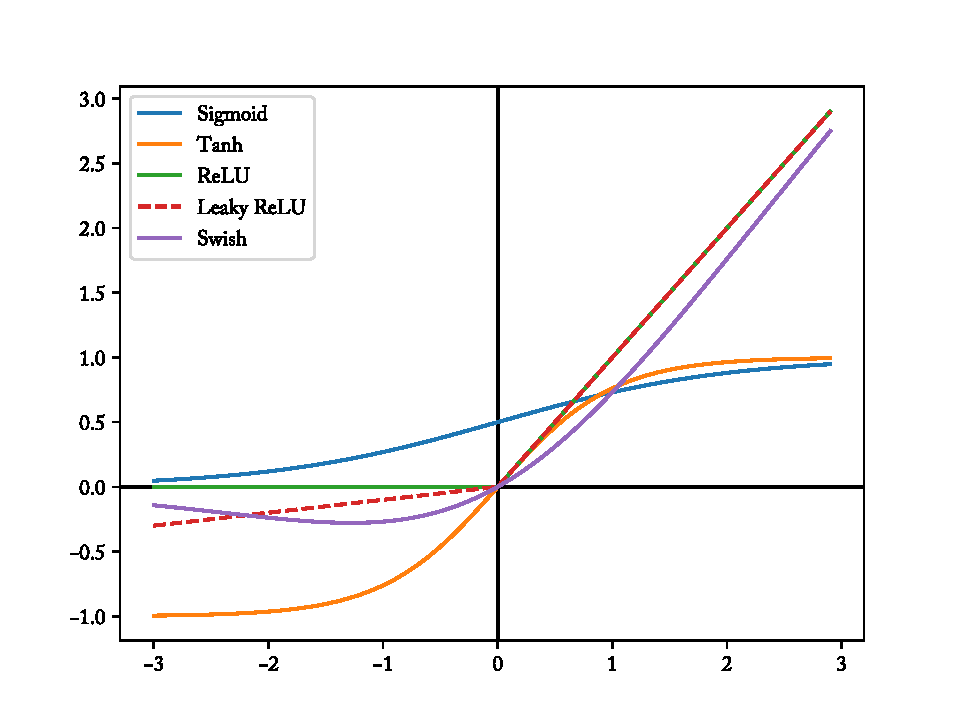
\includegraphics[width=0.7\paperwidth]{activation_fun_comparison}}
	\caption{Comparison of activation functions}
	\label{fig:activation_functions}
\end{figure}

Some important trends have been discovered by \textit{Searching for Activation Functions} \cite{DBLP:journals/corr/abs-1710-05941}, a recent study using automated search and benchmarking techniques:

\begin{enumerate}
	\item Complicated activation functions consistently underperform simpler activation functions;
	\item A common structure shared by the top activation functions is the use of the raw preactivation $x$ as input to the final binary function;
	\item Functions that use division tend to perform poorly because the output explodes when the denominator approaches zero.
\end{enumerate}

\section{Loss Functions}

\subsection{Regression loss}

\begin{equation}
	L_2(y, \hat{y}) = MSE = \sum\limits_{i=1}^n  {(y_i - \hat{y}_i)}^2
\end{equation}

\begin{equation}
	L_1(y, \hat{y}) = MAE = \sum\limits_{i=1}^n  {|y_i - \hat{y}_i|}
\end{equation}

\begin{equation}
	L_{cosh}(y, \hat{y}) = \sum\limits_{i=1}^n  {\log(\cosh(\hat{y}_i-y_i))}
\end{equation}

\begin{equation}
	L_\gamma(y, \hat{y}) = \sum\limits_{i=y_i<\hat{y}_i}  ({\gamma-1}).|y_i - \hat{y}_i| + \sum\limits_{i=y_i\geq \hat{y}_i}  ({\gamma}).|y_i - \hat{y}_i|
\end{equation}



\begin{figure}
	\centerline{
		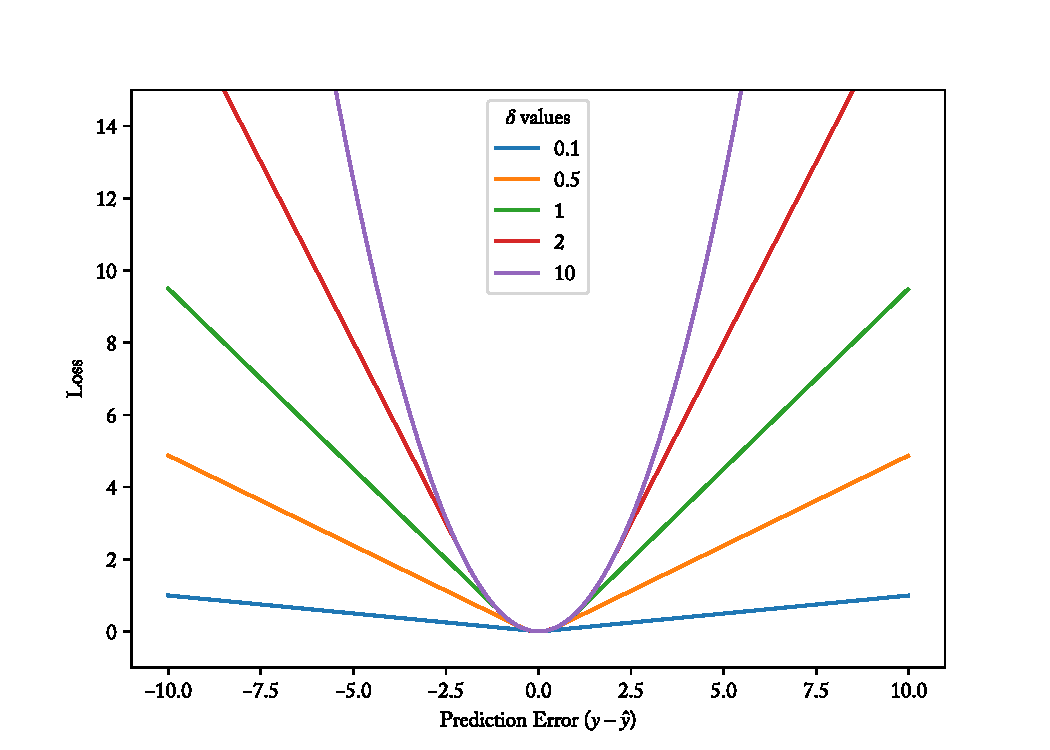
\includegraphics[width=0.6\paperwidth]{loss_Huber}}
	\caption{Huber/Smooth MAE Loss Function using various $\delta$ values}
	\label{fig:Loss Huber}
\end{figure}

\begin{figure}
	\centerline{
		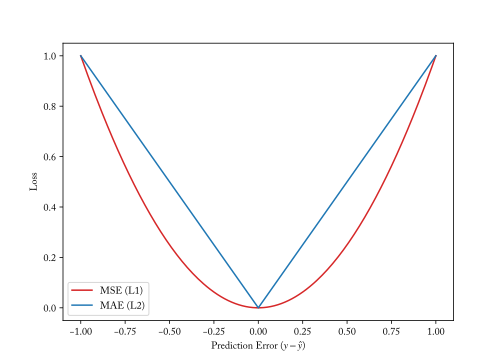
\includegraphics[width=0.6\paperwidth]{loss_L1_L2}}
	\caption{Mean Square Error (L2) vs Mean Absolute Error (L1) Loss Functions}
	\label{fig:Loss L1 L2}
\end{figure}

\begin{figure}
	\centerline{
		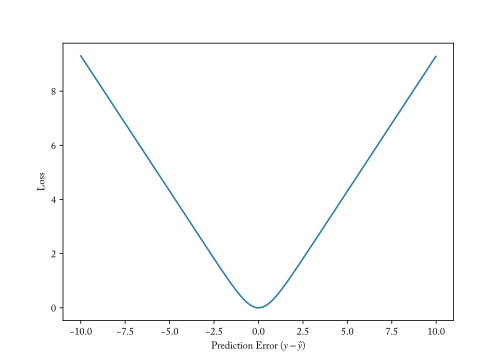
\includegraphics[width=0.6\paperwidth]{loss_logcosh}}
	\caption{Log-Cosh Loss Function}
	\label{fig:Loss L1 L2}
\end{figure}

\begin{figure}
	\centerline{
		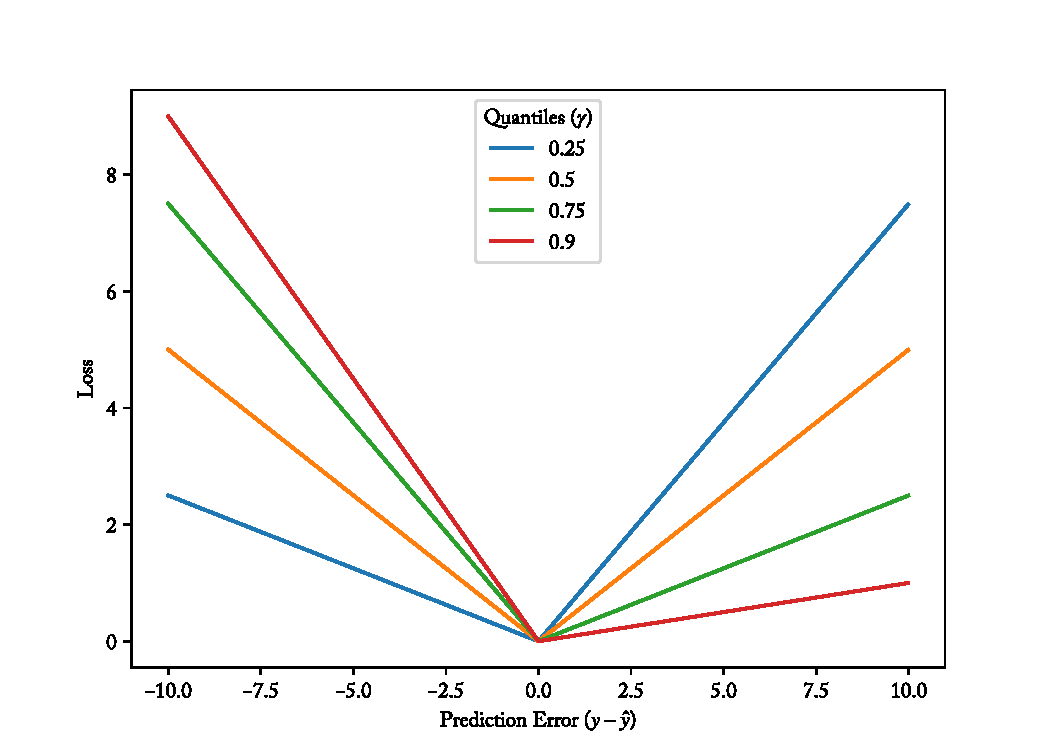
\includegraphics[width=0.6\paperwidth]{loss_quant}}
	\caption{Quantile Loss Function, with different Quantiles ($\gamma$) values}
	\label{fig:Loss L1 L2}
\end{figure}

\subsection{Classification loss}